
% v2-acmsmall-sample.tex, dated March 6 2012
% This is a sample file for ACM small trim journals
%
% Compilation using 'acmsmall.cls' - version 1.3 (March 2012), Aptara Inc.
% (c) 2010 Association for Computing Machinery (ACM)
%
% Questions/Suggestions/Feedback should be addressed to => "acmtexsupport@aptaracorp.com".
% Users can also go through the FAQs available on the journal's submission webpage.
%
% Steps to compile: latex, bibtex, latex latex
%
% For tracking purposes => this is v1.3 - March 2012
\documentclass[prodmode,acmtecs]{acmsmall} % Aptara syntax
\usepackage[spanish,polish]{babel}
\usepackage[T1]{fontenc}
\usepackage{fancyvrb}
\usepackage{graphicx,hyperref}
\newcommand\cutout[1]{}


\usepackage[table]{xcolor}
\usepackage[utf8]{inputenc}
\usepackage[parfill]{parskip}
\usepackage{tabulary}
\PassOptionsToPackage{hyphens}{url}
\usepackage{hyperref}    
\usepackage[capitalize]{cleveref}


% Metadata Information
% !!! TODO: SET THESE VALUES !!!
\acmVolume{0}
\acmNumber{0}
\acmArticle{CFP}
\acmYear{0}
\acmMonth{0}

\newcounter{colstart}
\setcounter{page}{4}

\RecustomVerbatimCommand{\VerbatimInput}{VerbatimInput}%
{
%fontsize=\footnotesize,
fontfamily=\rmdefault
}


\newcommand{\UnderscoreCommands}{%\do\verbatiminput%
\do\citeNP \do\citeA \do\citeANP \do\citeN \do\shortcite%
\do\shortciteNP \do\shortciteA \do\shortciteANP \do\shortciteN%
\do\citeyear \do\citeyearNP%
}

\usepackage[strings]{underscore}



% Document starts
\begin{document}


\setcounter{colstart}{\thepage}

\acmArticle{CFP}
\title{{\huge\sc SIGLOG Monthly 243}

 November 2023}
\author{DAVID PURSER\affil{University of Liverpool, UK}
\vspace*{-2.6cm}\begin{flushright}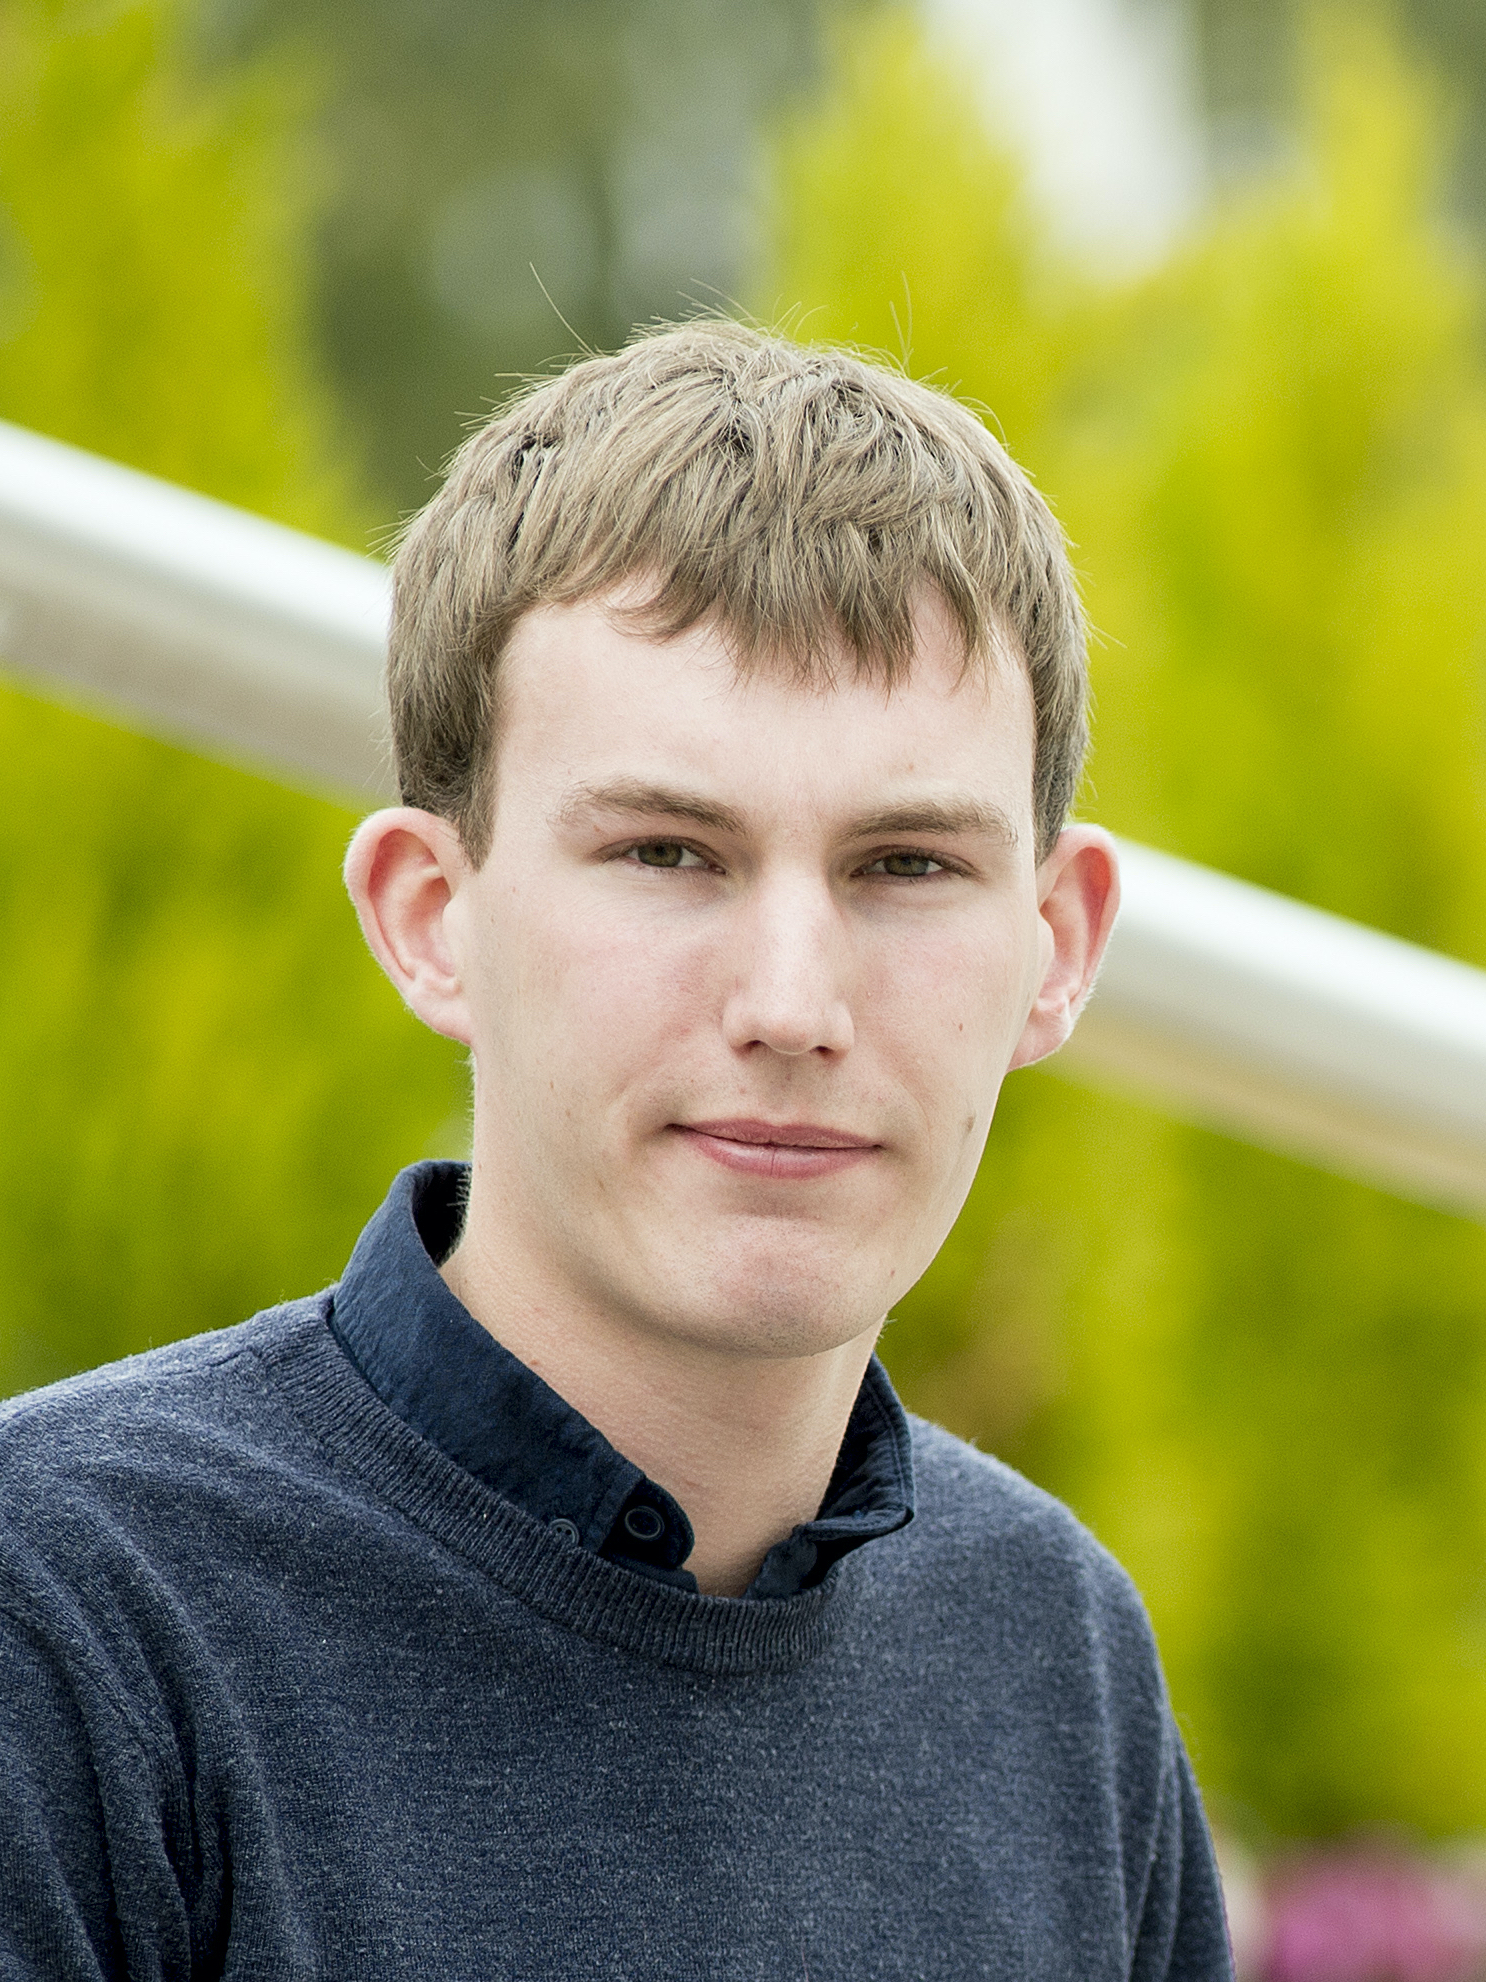
\includegraphics[width=30mm]{dp}\end{flushright}
}

\begin{abstract}
November 2023 edition of SIGLOG Monthly, featuring deadlines, calls and community announcements.
\end{abstract}


\maketitlee

\href{https://lics.siglog.org/newsletters/}{Past Issues}
 - 
\href{https://lics.siglog.org/newsletters/inst.html}{How to submit an announcement}
\section{Table of Content}\begin{itemize}\item DEADLINES (\cref{deadlines}) 
 
\item CALLS 
 
\begin{itemize}\item CTLM 2023 (CALL FOR PARTICIPATION) (\cref{CTLM2023})
\item IJCAR 2024 (CALL FOR PAPERS, CALL FOR CO-LOCATED EVENTS) (\cref{IJCAR2024})
\item CAV 2024 (CALL FOR PAPERS) (\cref{CAV2024})
\item CiE 2024 (CALL FOR PAPERS) (\cref{CiE2024})
\item ICALP 2024 (CALL FOR PAPERS) (\cref{ICALP2024})
\item AiML 2024 (CALL FOR PAPERS) (\cref{AiML2024})
\end{itemize} 
\item JOB ANNOUNCEMENTS 
 
\begin{itemize}\item PhD scholarship in Computer Science in Paris (\cref{PhDscholarshipinComputerScienceinParis})
\item PhD position in Logic and Legal Reasoning at TU Wien (\cref{PhDpositioninLogicandLegalReasoningatTUWien})
\item Postdoctoral opportunities in verification/synthesis for AI at Oxford (\cref{PostdoctoralopportunitiesinverificationsynthesisforAIatOxford})
\item Postdoctoral Research Associate In Verification at Liverpool (\cref{PostdoctoralResearchAssociateInVerificationatLiverpool})
\end{itemize} 
\end{itemize}\section{Deadlines}\label{deadlines}\rowcolors{1}{white}{gray!25}\begin{tabulary}{\linewidth}{LL}2 Postdocs in verification/synthesis for AI at Oxford:  & Nov 06, 2023 (Applications) \\
CTLM 2023:  & Nov 07, 2023 (Contributed talks) \\
Postdoc in Verification and Game Theory at Liverpool:  & Nov 10, 2023 (Applications) \\
PhD in Logic and Legal Reasoning at TU Wien:  & Nov 30, 2023 (Applications) \\
FLOPS 2024:  & Dec 06, 2023 (Abstract), Dec 13, 2023 (Papers) \\
4 Positions at Oxford:  & Dec 13, 2023 (Deadline) \\
DEON2023:  & Jan 07, 2024 (Paper) \\
SPIN 2024:  & Jan 15, 2024 (Submissions) \\
IJCAR 2024:  & Jan 15, 2024 (Abstract), Jan 22, 2024 (Paper), Nov 27, 2023 (Co-located event proposals) \\
CAV 2024:  & Jan 19, 2024 (Paper), Mar 01, 2024 (CAV Award Nomination deadline) \\
LICS 2024:  & Jan 21, 2024 (Titles and Short Abstracts), Jan 26, 2024 (Full Papers Due) \\
FSCD 2024:  & Feb 05, 2024 (Abstract), Feb 12, 2024 (Paper) \\
CiE 2024:  & Feb 10, 2024 (Article), May 15, 2024 (Informal presentations) \\
ICALP 2024:  & Feb 14, 2024 (Paper) \\
AiML 2024:  & Mar 08, 2024 (Abstract), Mar 15, 2024 (Full papers) \\
\end{tabulary}
\section{CTLM 2023: Conference on Techniques from Logic in Mathematics }\label{CTLM2023}  TU Wien, Vienna, Dec 7, 2023\\ 
CALL FOR PARTICIPATION 

\begin{itemize}\item  We are organizing a one-day conference at TU Wien on Dec 7, 2023, focusing mainly on the connection between logic and other mathematics. 
 
  We have two invited speakers, Julia Wolf (University of Cambridge, UK) and Ulrich Kohlenbach (TU Darmstadt, Germany). 
 
  Now we are looking for contributed speakers and we'd appreciate if you take into consideration giving a talk at the conference. 
 
  The deadline for submitting your presentation proposal (the title and abstract of your talk) is Nov 7, 2023. 
 
  For more information, please visit \href{https://sites.google.com/view/techniquesfromlogic/home}{https://sites.google.com/view/techniquesfromlogic/home}. If you have any questions, you may contact Lorenzo Sauras-Altuzarra (lorenzo@logic.at). Thank you in advance. 
 
\end{itemize}\section{IJCAR 2024: The 12th International Joint Conference on Automated Reasoning}\label{IJCAR2024}  Nancy, France, July 1-6, 2024\\ 
  \href{https://ijcar2024.loria.fr/}{https://ijcar2024.loria.fr/}\\ 
CALL FOR PAPERS 

\begin{itemize}\item  IJCAR is the premier international joint conference on all topics in automated reasoning.  
 
  IJCAR 2024 will be hosted by the Inria Nancy Research Center and LORIA in Nancy, France, from July 1-6, 2024. 
 
  IJCAR 2024 is the merger of leading events in automated reasoning: 
 
\begin{itemize}\item  CADE (Conference on Automated Deduction)
\item  FroCoS (Symposium on Frontiers of Combining Systems)
\item  TABLEAUX (Conference on Analytic Tableaux and Related Methods)
\end{itemize} 
\item  TOPICS 
 
  IJCAR 2024 invites submissions related to all aspects of automated or interactive logical reasoning, including foundations, implementations, and applications. Original research papers and descriptions/evaluations of working automated deduction systems or proof assistant systems are solicited.  
 
  IJCAR topics include the following: 
 
\begin{itemize}\item  Logics of interest include: propositional, first-order, classical, equational, higher-order, non-classical, constructive, modal, temporal, many-valued, substructural, description, type theory.
\item  Methods of interest include: tableaux, sequent calculi, resolution, model-elimination, inverse method, paramodulation, term rewriting, induction, unification, constraint solving, decision procedures, model generation, model checking, semantic guidance, interactive theorem proving, logical frameworks, AI-related methods for deductive systems, proof presentation, automated theorem proving, combination of decision or proof procedures, SAT and SMT solving, machine learning and theorem proving, integration of automated provers/proof assistants in automated test generators, program synthesisers, verified compilers, intelligent systems, agent based systems, knowledge processing systems, formal methods tools and other symbolic tools, etc.
\item  Applications of interest include: verification, formal methods, program analysis and synthesis, computer mathematics, declarative programming, deductive databases, knowledge representation and processing/engineering, education, formalization of mathematics, trusted AI, etc.
\end{itemize} 
\item  IMPORTANT DATES (partly tentative) 
 
\rowcolors{1}{white}{gray!25}\begin{tabulary}{\linewidth}{LL}Abstract submission:  & Jan 15, 2024 \\
Paper submission:  & Jan 22, 2024 \\
Notification of paper decisions (tentative):  & Mar 15, 2024 \\
Camera-ready papers due (tentative):  & Apr 04, 2024 \\
Workshops \& Tutorials:  & Jul 1-2, 2024 \\
Conference, including CASC:  & Jul 3-6, 2024 \\
\end{tabulary}
 
\item  WORKSHOPS, TUTORIALS, SYSTEM COMPETITION 
 
  A two-day workshop and tutorial programme will be co-organized with the conference. In addition, the annual CADE ATP System Competition (CASC) will be held during the conference. Details will be published in separate calls and on the conference website. 
 
\item  SUBMISSION GUIDELINES 
 
  Please see full call: \href{https://merz.gitlabpages.inria.fr/2024-ijcar/post/call-for-papers/}{https://merz.gitlabpages.inria.fr/2024-ijcar/post/call-for-papers/} 
 
\item  BEST PAPER AWARD 
 
  IJCAR 2024 will recognize the most outstanding submissions with a best paper award and a best student paper award at the conference. 
 
\item  STUDENT TRAVEL AWARDS 
 
  Woody Bledsoe Travel Awards will be available to support selected students in attending the conference. 
 
\end{itemize}CALL FOR CO-LOCATED EVENTS 

\begin{itemize}\item  The International Joint Conference on Automated Reasoning (IJCAR 2024) is soliciting proposals for co-located events such as workshops, tutorials and competitions. 
 
  Researchers are invited to submit proposals on any topic related to automated reasoning, from theoretical foundations to tools and applications. 
 
  The co-located events will take place before the IJCAR conference on Monday \& Tuesday, July 1-2, 2024. 
 
  Proposals can have up to three pages and should consist of the following two parts. 
 
\begin{itemize}\item  A description part including: short scientific justification of the proposed topic, its significance, and the particular benefits of the workshop to the community, as well as a list of previous or related workshops (if relevant); and a brief description (up to 120 words) of the event for the website and publicity material.
\item  An organisational part including: contact information for the workshop organisers; proposed affiliated conference; estimate of the number of workshop participants; proposed format and agenda (e.g. paper presentations, tutorials, demo, sessions, etc.) potential invited speakers; procedures for selecting papers and participants; tentative schedule for paper submission and notification of acceptance; plans (and needs) for remote participation [A zoom connection can be provided on demand]; plans for dissemination, if any (e.g. a journal special issue); duration (which may vary from one day to two days); and any other special requirements.
\end{itemize} 
  The organisers of co-located events are expected to create and maintain a website for the event; handle paper selection, reviewing and acceptance; draw up a tentative programme of talks; advertise their event through specialist mailing lists; prepare the informal pre-proceedings (if applicable) in a timely fashion; plan for remote participation (if applicable); and arrange post-proceedings if any. 
 
  The IJCAR organising committee will handle promotion of the event on the main conference website; integration of the event's programme into the overall timetable; registration of participants; arrangement of an appropriate meeting room; and provision of lunch and coffee breaks for participants. 
 
  Proposals should be sent directly to Sophie Tourret by email at sophie.tourret@inria.fr 
 
\item  IMPORTANT DATES 
 
\rowcolors{1}{white}{gray!25}\begin{tabulary}{\linewidth}{LL}Co-located event proposals submission:  & Nov 27, 2023 \\
Notification of success of proposals:  & Dec 11, 2023 \\
Main conference:  & Jul 3-6, 2024 \\
Workshop dates:  & Jul 1-2, 2024 \\
\end{tabulary}
 
\end{itemize}\section{CAV 2024: 36th International Conference on Computer-Aided Verification}\label{CAV2024}  July 22-27 2024, Montreal, Canada\\ 
  \href{http://i-cav.org/2024/call-for-papers/}{http://i-cav.org/2024/call-for-papers/}\\ 
CALL FOR PAPERS 

\begin{itemize}\item CONFERENCE 
 
  CAV 2024 is the 36th in a series dedicated to the advancement of the theory and practice of computer-aided formal analysis methods for hardware and software systems. The conference covers the spectrum from theoretical results to concrete applications, with an emphasis on practical verification tools and the algorithms and techniques that are needed for their implementation. CAV considers it vital to continue spurring advances in hardware and software verification while expanding to new domains such as machine learning, autonomous systems, and computer security. The proceedings of the conference will be published in the Springer-Verlag Lecture Notes in Computer Science series. A selection of papers is expected to be invited to a special issue of Formal Methods in System Design and the Journal of the ACM. 
 
\item  TOPICS 
 
  Topics of interest include but are not limited to: Algorithms and tools for verifying models and implementations; Algorithms and tools for system synthesis; Algorithms and tools that combine verification and learning; Mathematical and logical foundations of verification and synthesis; Specifications and correctness criteria for programs and systems; Deductive verification using proof assistants; Hardware verification techniques; Program analysis and software verification; Software synthesis; Hybrid systems and embedded systems verification; Formal methods for cyber-physical systems; Compositional and abstraction-based techniques for verification; Probabilistic and statistical approaches to verification; Verification methods for parallel and concurrent systems; Testing and run-time analysis based on verification technology; Decision procedures and solvers for verification and synthesis; Applications and case studies in verification and synthesis; Verification in industrial practice; New application areas for algorithmic verification and synthesis; Formal models and methods for security; Formal models and methods for biological systems  
 
    Submissions on a wide range of topics are sought, particularly ones that identify new research directions. CAV 2024 is not limited to topics discussed in previous instances of the conference. Authors concerned about the appropriateness of a topic may communicate with the conference chairs prior to submission. 
 
\item  SUBMISSION 
 
  Main submission site is: \href{https://easychair.org/conferences/?conf=cav2024}{https://easychair.org/conferences/?conf=cav2024}.  
 
  Paper submissions in CAV fall into one of the following three categories (more information here: \href{http://i-cav.org/2024/call-for-papers/}{http://i-cav.org/2024/call-for-papers/}): 
 
\begin{itemize}\item  Regular Papers (18 pages max, must be anonymized) 
\item  Tool Papers (10 pages max, not anonymized) 
\item  Industrial Experience Reports \& Case Studies. (10 pages max, not anonymized) 
\end{itemize} 
  Papers in all three categories must be submitted by January 19th, 2024 AoE, and should be in LNCS format. Simultaneous submission to other conferences with proceedings or submission of material that has already been published elsewhere is not allowed. The review process will include a feedback/rebuttal period where authors will have the option to respond to reviewer comments. The PC chairs may solicit further reviews after the rebuttal period.  
 
\item  IMPORTANT DATES (AoE) 
 
\rowcolors{1}{white}{gray!25}\begin{tabulary}{\linewidth}{LL}Paper submission:  & Jan 19, 2024 \\
Rebuttal period:  & Feb 29-Mar 3, 2024 \\
Author notification:  & Mar 26, 2024 \\
Artifact submission:  & Apr 8, 2024 (mandatory for tool papers) \\
Artifact notification:  & May 10, 2024 \\
Final version due:  & May 19, 2024 \\
Workshops:  & Jul 22-23, 2024 \\
Main Conference:  & Jul 24-27, 2024 \\
\end{tabulary}
 
\item  CAV AWARD  
 
  The CAV award is given annually at the CAV conference for fundamental contributions to the field of Computer-Aided Verification. For details about the CAV award nomination, please see the following page: \href{http://i-cav.org/2024/cav-award/}{http://i-cav.org/2024/cav-award/}. 
 
CAV Award Nomination deadline: Mar 01, 2024 
 
\item  CONTACT (CONFERENCE CO-CHAIRS) 
 
\begin{itemize}\item  Arie Gurfinkel, University of Waterloo 
\item  Vijay Ganesh, Georgia Tech
\end{itemize} 
\end{itemize}\section{CiE 2024: Computability in Europe 2024 Twenty years of theoretical and practical synergies}\label{CiE2024}  Amsterdam, The Netherlands, July 08-12, 2024\\ 
  \href{https://events.illc.uva.nl/CiE/CiE2024/}{https://events.illc.uva.nl/CiE/CiE2024/}\\ 
CALL FOR PAPERS 

\begin{itemize}\item  IMPORTANT DATES (AOE): 
 
\rowcolors{1}{white}{gray!25}\begin{tabulary}{\linewidth}{LL}Article submission:  & Feb 10, 2024 \\
Notification of acceptance:  & Apr 20, 2024 \\
Final versions due:  & May 01, 2024 \\
Informal presentations submission:  & May 15, 2024 \\
Early registration before:  & May 20, 2024 \\
Conference:  & July 08-12, 2024 \\
\end{tabulary}
 
  The notifications of acceptance for informal presentations will be sent a few days after submission. 
 
\item  GENERAL INFORMATION 
 
  CiE 2024 will be an anniversary event. It is the 20th conference organized by CiE (Computability in Europe), in the same place as the first edition, Amsterdam. 
 
  CiE is a European association of mathematicians, logicians, computer scientists, philosophers, physicists and others interested innew developments in computability and their underlying significance for the real world. 
 
\item  TUTORIAL SPEAKERS 
 
\begin{itemize}\item  Matthew Harrison-Trainor (University of Illinois Chicago)
\item  Sonja Smets (University of Amsterdam)
\end{itemize} 
\item  INVITED SPEAKERS 
 
\begin{itemize}\item  Arnold Beckmann (Swansea University)
\item  Rod Downey (Victoria University of Wellington)
\item  Elvira Mayordomo (University of Zaragoza)
\item  Alexandre Miquel (Universidad de la República)
\item  Monika Seisenberger (Swansea University)
\item  Mariya Soskova (University of Wisconsin–Madison)
\end{itemize} 
\item  SPECIAL SESSIONS 
 
  There will be 6 special sessions, including: 
 
\begin{itemize}\item  Computable aspects of symbolic dynamics and tilings (chairs: Benjamin Hellouin and Ilkka Torma)
\item  Algorithmic randomness and Kolmogorov complexity session (chairs: Rupert Hölzl abd Denis Hirschfeldt)
\item  Bio-inspired Computation (BiC)
\item  History and Philosophy of Computing (HaPoC)
\end{itemize} 
  Other topics of the special sessions will be announced soon. 
 
\item  CONFERENCE TOPICS 
 
  See full call for submission instructions: \href{https://events.illc.uva.nl/CiE/CiE2024/Submissions/}{https://events.illc.uva.nl/CiE/CiE2024/Submissions/} 
 
\item  INFORMAL PRESENTATIONS 
 
  Continuing the tradition of past CiE conferences, we invite researchers to present informal presentations of their recent work. A proposal for an informal presentation must be submitted via e-mail (e.pimentel@ucl.ac.uk), using the LNCS style file (available at \href{https://www.springer.com/gp/computer-science/lncs/conference-proceedings-guidelines}{https://www.springer.com/gp/computer-science/lncs/conference-proceedings-guidelines}), and be 1 page long; a brief description of the results suffices and an abstract is not required. Informal presentations will not be published in the LNCS conference proceedings. Results presented as informal presentations at CiE 2024 may appear or may have appeared in other conferences with formal proceedings and/or in journals. 
 
\item  WOMEN IN COMPUTABILITY 
 
  We are very happy to announce that within the framework of the Women in Computability program, we are able to offer some grants for junior women researchers who want to participate in CiE 2024. Applications for this grant should be sent to Lorenzo Galeotti <l.galeotti@uva.nl>, before May 15, 2024 and include a short cv (at most 2 pages) and contact information for an academic reference. Preference will be given to junior women researchers who are presenting a paper (including informal presentations) at CiE 2024. 
 
\item  HOSTED BY 
 
  The event will be held in the Amsterdam University College academic building located at Amsterdam Science Park. We are grateful for support from the University of Amsterdam. 
 
\end{itemize}\section{ICALP 2024: The 51st EATCS International Colloquium on Automata, Languages, and Programming}\label{ICALP2024}  Tallinn, Estonia, July 8-12, 2024\\ 
  \href{https://compose.ioc.ee/icalp2024/}{https://compose.ioc.ee/icalp2024/}\\ 
CALL FOR PAPERS 

\begin{itemize}\item  ICALP is the main conference and annual meeting of the European Association for Theoretical Computer Science (EATCS). As usual, ICALP will be preceded by a series of workshops, which will take place on July 7. 
 
  The 2024 edition has the following features: 
 
\begin{itemize}\item  Submissions are anonymous and there is a rebuttal phase.
\item  The conference is planned as a physical, in-person event.
\item  ICALP 2024 is co-located with Logic in Computer Science (LICS) 2024 and  Formal Structures for Computation and Deduction (FSCD) 2024.
\end{itemize} 
\item  Important dates and information 
 
\rowcolors{1}{white}{gray!25}\begin{tabulary}{\linewidth}{LL}Submissions:  & Feb 14, 2024 (1pm CET) \\
Rebuttal:  & Mar 26-29, 2024 \\
Author notification:  & Apr 14, 2024 \\
Camera-ready version:  & Apr 28, 2024 \\
Early registration:  & TBA \\
Conference:  & Jul 8-12, 2024 (Workshops on July 7) \\
\end{tabulary}
 
  Deadlines are firm; late submissions will not be considered. 
 
\item  SUBMISSION GUIDELINES 
 
  Please see full call for submission guidance. 
 
\item  AWARDS 
 
  During the conference, the following awards will be delivered: 
 
\begin{itemize}\item  the EATCS award,
\item  the Gödel prize,
\item  the Presburger award,
\item  the EATCS distinguished dissertation award,
\item  the best papers for Track A and Track B,
\item  the best student papers for Track A and Track B.
\end{itemize} 
\item  Proceedings 
 
  Published open access in Leibniz International Proceedings in Informatics (LIPIcs). 
 
\item  TOPICS 
 
\begin{itemize}\item  Track A: Algorithms, Complexity and Games: Algorithmic and Complexity Aspects of Network Economics; Algorithmic Aspects of Biological and Physical Systems; Algorithmic Aspects of Networks and Networking; Algorithmic Aspects of Security and Privacy; Algorithmic Game Theory and Mechanism Design; Approximation and Online Algorithms; Combinatorial Optimization; Combinatorics in Computer Science; Computational Complexity; Computational Geometry; Computational Learning Theory; Cryptography; Data Structures; Design and Analysis of Algorithms; Distributed and Mobile Computing; Foundations of Machine Learning; Graph Mining and Network Analysis; Parallel and External Memory Computing; Parameterized Complexity; Quantum Computing; Randomness in Computation; Sublinear Time and Streaming Algorithms; Theoretical Foundations of Algorithmic Fairness
\item  Track B: Automata, Logic, Semantics, and Theory of Programming: Algebraic and Categorical Models of Computation; Automata, Logic, and Games; Database Theory, Constraint Satisfaction Problems, and Finite Model Theory; Formal and Logical Aspects of Learning; Formal and Logical Aspects of Security and Privacy; Logic in Computer Science and Theorem Proving; Models of Computation: Complexity and Computability; Models of Concurrent, Distributed, and Mobile Systems; Models of Reactive, Hybrid, and Stochastic Systems; Principles and Semantics of Programming Languages; Program Analysis, Verification, and Synthesis; Type Systems and Typed Calculi
\end{itemize} 
\end{itemize}\section{AiML 2024: 15th International Conference on Advances in Modal Logic}\label{AiML2024}  19-23 Aug 2024 | Prague\\ 
CALL FOR PAPERS 

\begin{itemize}\item  Advances in Modal Logic is an initiative aimed at presenting the state of the art in modal logic and its various applications. The initiative consists of a conference series together with volumes based on the conferences. 
 
  There will be two types of submissions for AiML 2024: 
 
\begin{itemize}\item  Full papers for publication in the proceedings and presentation at the conference.
\item  Short presentations intended for presentation at the conference but not for the published proceedings.
\end{itemize} 
  Both types of papers should be submitted electronically using the EasyChair submission page starting from January 29th, 2024. 
 
  For more information, please visit \href{https://www.cs.cas.cz/aiml2024/cfp.html}{https://www.cs.cas.cz/aiml2024/cfp.html} 
 
\item  IMPORTANT DATES 
 
\rowcolors{1}{white}{gray!25}\begin{tabulary}{\linewidth}{LL}Abstract submission:  & Mar 08, 2024 \\
Full papers submission:  & Mar 15, 2024 \\
Full papers notification:  & May 20, 2024 \\
Short presentations submission:  & May 30, 2024 \\
Short presentations notification:  & Jun 14, 2024 \\
Final versions of full papers and short presentations:  & Jun 21, 2024 \\
Registration deadline:  & TBA \\
Conference:  & Aug, 19–22 2024 \\
\end{tabulary}
 
\end{itemize}\section{PhD scholarship in Computer Science in Paris: Model Checking for Malware (Virus) Detection}\label{PhDscholarshipinComputerScienceinParis}JOB ANNOUNCEMENT 

\begin{itemize}\item  A PhD  position is available in  the  Laboratoire d’Informatique de Paris-Nord (LIPN), Villetaneuse, France. Contact: Tayssir TOUILI  (touili@lipn.fr) 
 
  The  recruited  PhD student  is expected to investigate and develop novel techniques, algorithms and tools for malware detection. The ultimate goal is to build a malware detector that beats the existing commercial malware detection tools. 
 
  More details can be found here: \href{https://lipn.univ-paris13.fr/~touili/sujet-PhD.pdf}{https://lipn.univ-paris13.fr/~touili/sujet-PhD.pdf} 
 
\item  How to apply: 
 
  The position is available immediately. Candidates must have a master in computer science and be  good programmers. The candidate must send a CV, university grades,  recommendation letters, and a motivation letter to Tayssir TOUILI (touili@lipn.fr)  
 
\end{itemize}\section{PhD position in Logic and Legal Reasoning at TU Wien}\label{PhDpositioninLogicandLegalReasoningatTUWien}  TU Wien, Faculty of Informatics, Vienna\\ 
JOB ANNOUNCEMENT 

\begin{itemize}\item  The research group Theory and Logic, Institute of Logic and Computation of the Vienna University of Technology is seeking an exceptionally talented and motivated student for a PhD position. 
 
  The position is embedded in the LoDEx project (Logical Methods for Deontic Explanations), a joint project between TU Wien (PI: Agata Ciabattoni), the University of Luxembourg (PI: Leon van der Torre), and the Ruhr-University Bochum (PI: Christian Straßer). 
 
  This PhD position is a shared position with the University of Luxembourg: the candidate is expected to spend the first two years at TU Wien in Vienna and then two years in Luxembourg completing his/her PhD under a Cotutelle agreement in the Computational Law and Machine Ethics (CLAiM) group at the University of Luxembourg. 
 
\item  Details: 
 
  \href{https://www.vcla.at/2023/10/phd-position-in-logic-and-legal-reasoning/}{https://www.vcla.at/2023/10/phd-position-in-logic-and-legal-reasoning/} 
 
  \href{https://www.ruhr-uni-bochum.de/lodex/}{https://www.ruhr-uni-bochum.de/lodex/} 
 
Apply before: Nov 30, 2023 
 
\end{itemize}\section{Postdoctoral opportunities in verification/synthesis for AI at Oxford}\label{PostdoctoralopportunitiesinverificationsynthesisforAIatOxford}JOB ANNOUNCEMENT 

\begin{itemize}\item   Two short-term postdoctoral positions area available on the FUN2MODEL project (fun2model.org), an ERC Advanced Grant (2019-2025) at the University of Oxford. Since the project has already advanced substantially and is currently developing new methodologies, priority will be given to researchers who are aligned with one or more of its six research themes (see \href{http://fun2model.org/researchthemes.php}{http://fun2model.org/researchthemes.php}): 
 
\begin{itemize}\item  Safety, Robustness and Fairness Guarantees \href{http://fun2model.org/safety.php}{http://fun2model.org/safety.php}
\item  Robustness Guarantees for Bayesian Neural Networks \href{http://fun2model.org/bayesian.php}{http://fun2model.org/bayesian.php}
\item  Efficient Robust Learning \href{http://fun2model.org/robust-learning.php}{http://fun2model.org/robust-learning.php}
\item  Tractable Causal Inference and Reasoning \href{http://fun2model.org/inference.php}{http://fun2model.org/inference.php}
\item  Multi-agent Coordination and Collaboration \href{http://fun2model.org/multi-agent.php}{http://fun2model.org/multi-agent.php}
\item  Human-like Decision Making \href{http://fun2model.org/human-like.php}{http://fun2model.org/human-like.php}
\end{itemize} 
  Please contact Marta Kwiatkowska at marta.kwiatkowska@cs.ox.ac.uk if you want to discuss. 
 
Application deadline: Nov 06, 2023 
 
  More information about the positions and the application process can be found at: \href{https://www.cs.ox.ac.uk/news/2193-full.html}{https://www.cs.ox.ac.uk/news/2193-full.html} 
 
\end{itemize}\section{Postdoctoral Research Associate In Verification at Liverpool}\label{PostdoctoralResearchAssociateInVerificationatLiverpool}JOB ANNOUNCEMENT 

\begin{itemize}\item  We are seeking to recruit a motivated and research-focused research associate to carry out research in Verification and Game Theory, as part of the EPSRC project ``Games for Good'' with Patrick Totzke, Sven Schewe and Qiyi Tang.  
 
  You will enjoy developing algorithms, lower bounds, and possibly proof-of-concept implementations related to computer-aided formal verification. The position includes collaboration with our academic partners and research visits across Europe.  
 
  The project aims to better understand the notion of good-for-games (GfG) and related restricted forms of non-determinism, especially for computational models with infinite state spaces. We will investigate new ways to restrict non-determinism that maintain high expressiveness while simultaneously allowing for efficient verification procedures. In particular, we plan to study stochastic variants of history-determinism, such as automata that are good-for-Markov chains / Markov Decision Processes, as well as stochastic resolvers and their memory requirements. As above, you will work together in collaboration with our partners to share research outputs and deliver results. 
 
\item  Further information: \href{https://www.jobs.ac.uk/job/DDK022/postdoctoral-research-associate-in-verification}{https://www.jobs.ac.uk/job/DDK022/postdoctoral-research-associate-in-verification} 
 
Application deadline: Nov 10, 2023 
 
\end{itemize}


\bigskip Links: \href{http://siglog.org/}{SIGLOG website}, \href{https://lics.siglog.org}{LICS website}, \href{https://lics.siglog.org/newsletters/}{SIGLOG Monthly}\end{document}